\documentclass{article}
\usepackage{graphicx}
\usepackage[margin=1.5cm]{geometry}
\usepackage{amsmath}

\begin{document}
\twocolumn

\title{Wednesday Warm Up: Unit 5: Momentum II}
\author{Prof. Jordan C. Hanson}

\maketitle

\section{Memory Bank}

\begin{itemize}
\item $v = r \omega$ ... Relationship between tangential velocity and angular velocity.
\item $\omega = 2\pi f = 2\pi/T$ ... Relationship between angular velocity ($\omega$), frequency ($f$), and period ($T$).
\item $\vec{p} = m\vec{v}$ ... Definition of momentum.
\item $\vec{F}_{\rm Net} = \frac{d\vec{p}}{dt}$ ... Force and momentum
\item Let $M$ be the total mass of a system, and let $m_j$ and $\vec{r}_j$ $(j = 1,...,N)$ be the masses and positions of the constituent parts of the system.  The position of the center of mass is
\begin{equation}
\vec{r}_{\rm CM} = \frac{1}{M}\sum_{j=1}^{N}m_j \vec{r}_j
\end{equation}
\item The momentum of the center of mass $\vec{P}_{\rm CM}$ is
\begin{equation}
\vec{P}_{\rm CM} = \sum_{j=1}^N \vec{p}_j
\end{equation}
\item The net external force on a system obeys
\begin{equation}
\vec{F} = \frac{d\vec{P}_{\rm CM}}{dt}
\end{equation}
\end{itemize}

\section{Momentum II}

\begin{enumerate}
\item Consider Fig. \ref{fig:1}, in which a single planet orbits a star located at the origin at $t=0$. Let the star have mass $M$, the planet have mass $m$, and let the distance between them be $r$.  Let the ratio of the masses be $\mu = m/M$.  (a) Show that the center of mass is given by 
\begin{equation}
\vec{r}_{\rm CM} = \left(\frac{\mu}{\mu+1}\right)\vec{r}
\end{equation}
(b) Show that $\vec{r} = 0$ in the limit that $\mu \ll 1$.
\\ \vspace{3cm}
\item Where is the center of mass if the star and the planet have the same mass? \\ \vspace{2cm}
\item Assume there is no \textit{net, external} force on the system.  The center of mass will
\begin{itemize}
\item A: Accelerate 
\item B: Decelerate
\item C: Remain stationary
\item D: Remain at constant velocity
\end{itemize}
\item Given the answer to the previous exercise, what do you conclude about the orbits of the star and planet? \\ \vspace{1cm}
\end{enumerate}

\begin{figure}[hb]
\centering
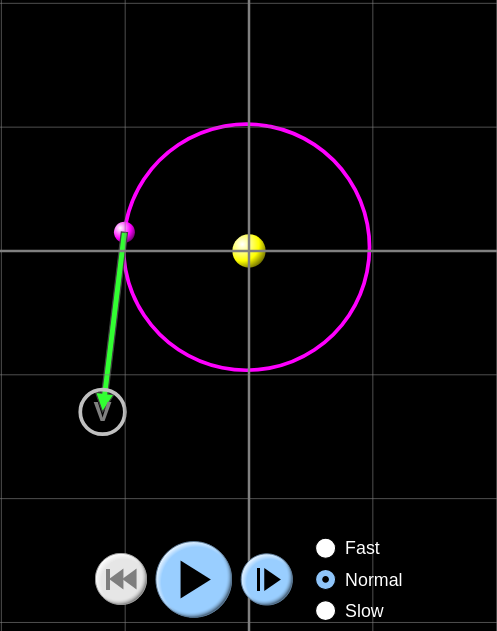
\includegraphics[width=0.33\textwidth]{figures/orbit.png}
\caption{\label{fig:1} A planet orbits a star.}
\end{figure}

\end{document}
